\documentclass[10pt,a4paper]{article}
\usepackage[latin1]{inputenc}
\usepackage{amsmath}
\usepackage{amsfonts}
\usepackage{amssymb}
\usepackage{hyperref}

\usepackage{graphicx}
\usepackage{listings}

\usepackage[margin=3cm]{geometry}

\author{Per Lenander, Anton Fosselius}
\title{ORSoC Graphics accelerator Specification}
\begin{document}

\maketitle

\begin{center}

\includegraphics[scale=1.0]{../pictures/OpenCores}
\end{center}

\begin{center}

\includegraphics[scale=0.50]{../pictures/wb_compatible}
\end{center}

\newpage

\section*{Revision history}
\begin{tabular}{|p{1cm}|p{2cm}|p{3cm}|p{7cm}|}
\hline \textbf{Rev.} & \textbf{Date} & \textbf{Author} & \textbf{Description} \\
\hline 
\hline 1.0 & 23/3/2012 & Per Lenander & Initial draft and basic functionality \\
\hline 2.0 & 4/6/2012 & Per Lenander & Advanced functionality (vector, 3D etc) \\
\hline 
\end{tabular} 
\newpage

\tableofcontents
\newpage

\section{Introduction}
The ORSoC Graphics accelerator allows the user to do advanced vector rendering and 2D blitting to a memory area. The core supports operations such as drawing textures, lines, curves and filling rectangular and triangular areas with color.

This IP Core is designed to integrate with the OpenRISC processor through a Wishbone bus interface. The core itself has no means of displaying the information rendered, for this purpose it can work alongside a display component, such as the enhanced VGA/LCD IP core found on OpenCores.

\subsection{Features}
\begin{itemize}
\item 32-bit Wishbone bus interface
\item Integrates with enhanced VGA/LCD IP core
\item Support for 16 bit color depth
\item Support for variable resolution
\item Acceleration of line operations
\item Acceleration of rectangle and triangle rasterization
\item Acceleration of memory copy operations
\item Textures can be saved to video memory
\item Vector transformation and rasterization
\item Clipping/Scissoring
\item Alpha blending and colorkeying
\item Filled Bezier curves
\item Bitmap Fonts
\item Vector Fonts (ttf)
\item Interpolation of colors  
\item UV-Mapping
\item Transformation (scaling and rotation)
\item 3D model support (.obj model files built using 3rd degree polygons)
\item Z-Buffer (triangles drawn in depth order)
\item Requires around 10000 Slice LUTs (Xilinx ISE 13.4)
\end{itemize}

\subsection{IP Core directory structure}
A overview of the contents of the IP core source folder can be found in figure \ref{fig:directory}.

\begin{figure}
\begin{center}
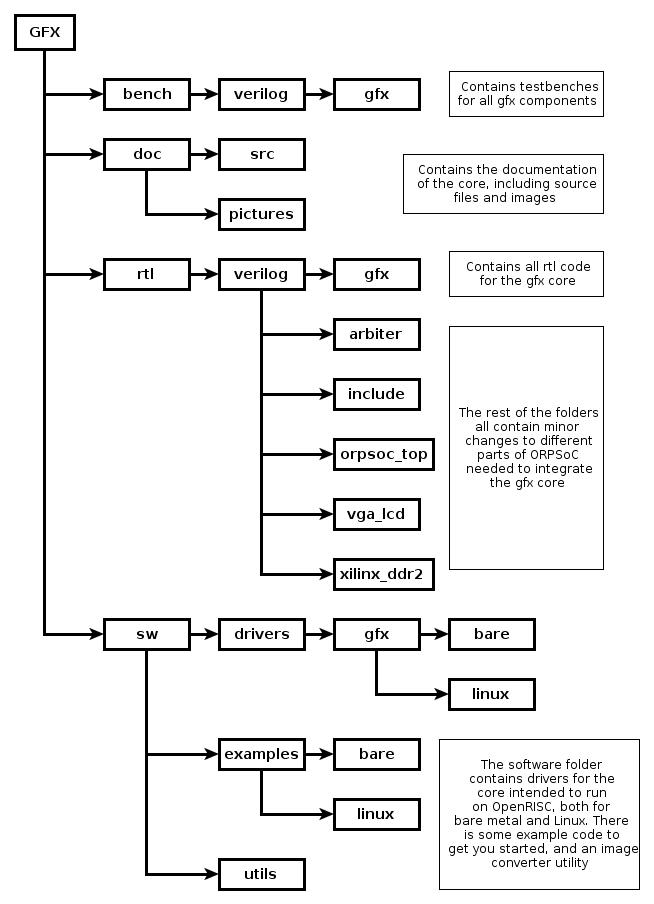
\includegraphics[scale=0.5]{../pictures/directory}
\caption{Directory structure of the ORSoC graphics accelerator.}
\label{fig:directory}
\end{center}
\end{figure}

\section{Architecture}
\subsection{Overview}
A topology of how the ORGFX is connected to the VGA driver and the OpenRISC core is shown in figure \ref{fig:topology}. The ORGFX has three wishbone interfaces: one read/write port that is used to communicate with the host CPU. One read port that reads depth/texture/alpha blending information from the RAM and one write port to write pixel information to the RAM.

\begin{figure}
\begin{center}
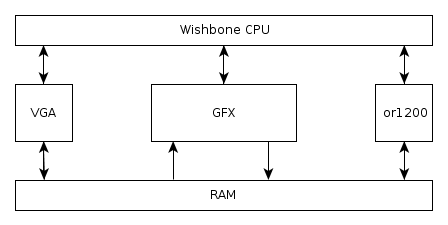
\includegraphics[scale=0.60]{../pictures/topology}
\caption{Overview of the ORPSoCv2's wishbone interconnection.}
\label{fig:topology}
\end{center}
\end{figure}

\subsection{Concepts}
This section describes a few basic terms used in this document.

\textbf{Video memory} -- The ORGFX component writes pixels one by one to an external memory, usually a SDRAM or DDR RAM chip. The CPU should also have access to this memory space to be able to write pixels directly (the easiest way to load textures).

\textbf{Render target} -- The render target, defined by the target base and size registers, describes the area to which all operations render pixels. It is possible to change the base address and size, enabling render-to-texture and double buffering.

\textbf{Surface/Texture} -- Any memory area that can be rendered to, including the render target, is considered a surface. A surface is defined by it's base address and size. There are two main surfaces that the ORGFX device handles: the render target and the currently active texture. Swapping between different textures has to be done in software. The operation of setting the current render target or texture is referred to as \textit{binding}.

\textbf{Source, Destination and Clip rectangles} -- There are three sets of rectangles that affect rendering, each described by two points. The first point sets the beginning of the rectangle, while the second point sets the pixel after the end of the rectangle. This way, a rectangle exactly filling the screen would be (0,0,640,480) at 640x480 resolution. See figure \ref{fig:SrcClipDest};

\textbf{Source rectangle} -- The source rectangle defines what pixels should be read from a texture during textured operations. The points are defined in the coordinates of the currently bound texture. This way sections of a texture can be drawn (good for tile maps or bitmap fonts).

\textbf{Destination rectangle} -- The destination rectangle defines where operations such as draw pixel and draw line will draw pixels, in the coordinates of the render target.

\textbf{Clip rectangle} -- The clip rectangle defines an area within the current render target which is valid to draw to. Any pixels outside this rectangle are discarded in the rasterization step. Pixels outside of the render target are automatically discarded.

\textbf{Z-buffer} -- The depth or Z-buffer is a surface containing z coordinate information. This can be used to draw graphics primitives in depth-correct order.

\begin{figure}
\begin{center}
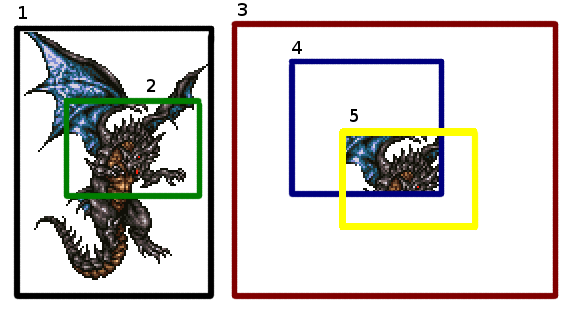
\includegraphics[scale=0.50]{../pictures/SrcClipDest}
\caption{1. Texture, 2. Source, 3. Render target, 4. Clip, 5. Destination}
\label{fig:SrcClipDest}
\end{center}
\end{figure}

\subsection{Coordinate precision}
The ORGFX core supports variable coordinate precision through two parameters, \textbf{point\_width} and \textbf{subpixel\_width}. Both parameters defaults to 16 bits width.

Target size, clip and source rects are defined as \textbf{point\_width} bit integers. Destination points are defined as fixed point numbers, with \textbf{point\_width} bit integer precision and \textbf{subpixel\_width} fractional precision. Internally many calculations are done with fixed point logic.

\subsection{Instruction FIFO}
All wishbone writes sent to the slave interface will pass through an instruction fifo. If the device is in the busy state (when the pipeline is active) the instruction will be queued instead of being set immediately. This is important to take into account when reading from registers, since an operation that changes the register being read might be queued. To find out if the device is busy, poll the status register and check if the busy bit is high.

\subsection{Pipeline}
The ORGFX core uses a pipelined architecture to speed up operation. An overview of the pipeline can be seen in figure \ref{fig:pipeline}. Each module in the pipeline communicates with acknowledge and write signals. A module will not assert write to the next module unless it receives an ack first (or if the module was previously in a ready state, in which case the downstream pipeline is empty). All ack and write signals are always exactly one clock tick long, to prevent triggering multiple instances of the same instruction.

Each module in the pipeline may hold the upstream pipeline for several clock ticks. For example, the rasterizer will prevent incoming raster instructions until all the pixels for the current operation are generated. When the rasterizer is ready for new data, it will send an ack upstream.

% The pipeline begins with the \textbf{transformation processor}, it calculates transformations like rotations and scaling. There after the next step in the pipeline is the \textbf{vector processor}, if there is no vector operations to be done, this step is skipped. When the vector calculations is done (if needed) the next step is the   \textbf{rasterizer}, its purpose is to convert points into pixels. When there are a request to write a rectangle, the \textbf{rasterizer} receives two points and outputs all the pixels between those points. The pixels generated by the \textbf{rasterizer} is recieved by the \textbf{fragment processor}. In the \textbf{fragment processor} the pixel gets a color either by a pre-set color or from a texture (via the \textbf{wishbone read} from the \textbf{memory}). The colored pixel is then sent to the \textbf{blender} which handles alpha blending. If alpha is enabled, the \textbf{blender} will read from the address in the \textbf{memory} where the pixel is going to be drawn. Then the new color is calculated based on the pixel color and the alpha value. The pixel is then passed on to the \textbf{renderer} which calculates the address in the memory where the pixel is going to be written. The pixel is then passed on to the \textbf{wishbone write} interface and finally to the render target in the \textbf{memory}.

\begin{figure}
\begin{center}
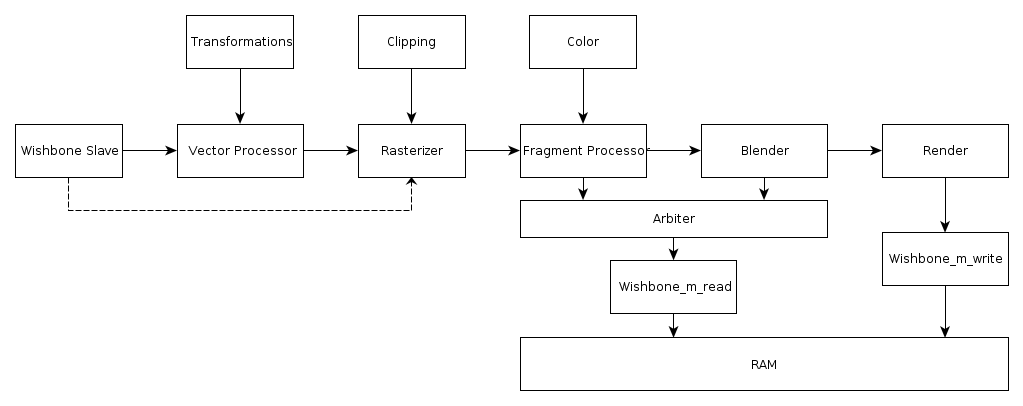
\includegraphics[scale=0.35]{../pictures/pipeline}
\caption{Picture of the ORGFX pipeline}
\label{fig:pipeline}
\end{center}
\end{figure}

\subsection{Description of core modules}

\subsubsection{Wishbone slave}
The wishbone slave handles all communication from the main OpenRISC processor (or other master CPU). This component holds all the registers, and the instruction FIFO that sets them. This component can be in one of two states: \textit{busy} or \textit{wait}. It enters the busy state when a pipeline operation is initialized, and returns to the wait state when the operation is finished. Operations can be initialized by writing to the control register (see section \ref{sec:registers}).

\subsubsection{Transformation processor}
The transformation processor handles rotations and scaling.

\subsubsection{Rasterizer}
This rasterizer generates pixel coordinates from points for several different operations.

\subsubsection{Clipper}
Discard generated pixel if clipping is enabled and pixel is out of bounds. Always discard pixels outside of the target area.

\subsubsection{Fragment processor}
The fragment processor adds color to the pixel generated by the rasterizer. If texturing is disabled, a color supplied from the color register is used. If texturing is enabled on the other hand, the u v coordinates supplied by the rasterizer are used to fetch a pixel from the active texture. If colorkeying is enabled and the fetched color matches the color key, the current pixel is discarded.

\subsubsection{Blender}
The blender module performs alpha blending if this is enabled. The module fetches the color of the pixel that the current operation will write to, and the mixes the value of the target color and the color from the fragment processor using the following algorithm:

\begin{quote}
$ alpha = alpha_{global} * alpha_{pixel} $

$ color_{out} = color_{in} * alpha + color_{target} * (1 - alpha) $
\end{quote}

Where alpha is a value between 0 (transparent) and 1 (opaque). If alpha blending is disabled the pixel is passed on unmodified. The alpha value can be interpolated over a triangle to create gradients. If this function is turned off (interpolation is disabled on triangle draws) then $alpha_{pixel}$ is set to 1.

\subsubsection{Wishbone arbiter}
Since two parts of the pipeline (fragment and blender) needs to access video memory, the arbiter makes certain only one of them can access the reader at once. The blender has the highest priority.

\subsubsection{Wishbone master read}
The wishbone reader handles all reads from video memory.

\subsubsection{Renderer}
The renderer calculates the memory address of the target pixel.

\subsubsection{Wishbone master write}
The wishbone master handles all writes to the video memory.

\section{IO Ports}
The Core has three wishbone interfaces:

\begin{itemize}
\item Wishbone slave -- connects to the data bus of the OpenRISC processor. In the case of ORPSoC, this bus is connected through an arbiter. Supports standard wishbone communications, not any burst modes.
\item Wishbone master read-only -- connects to a video memory port with read access. Used for fetching textures and during blending.
\item Wishbone master write-only -- connects to a video memory port with write access. Used for rendering pixels to the framebuffer.
\end{itemize}

There is an interrupt enabled that can be connected to the interrupt pins on the or1200 CPU (in the supplied orpsoc\_top it is connected to or1200\_pic\_ints[9]). For this interrupt to trigger, the correct bits in the control register has to be set.

\section{Registers}
\label{sec:registers}
\begin{tabular}{|l|l|l|l|l|}
\hline \textbf{Name} & \textbf{Addr} & \textbf{Width} & \textbf{Access} & \textbf{Description} \\ 
\hline
\hline CONTROL         & 0x00 & 32 & RW & Control register \\
\hline STATUS          & 0x04 & 32 & R  & Status register \\
\hline ALPHA           & 0x08 & 32 & RW & Global alpha register \\
\hline COLORKEY        & 0x0c & 32 & RW & Colorkey register \\

\hline TARGET\_BASE    & 0x10 & 32 & RW & Render target base \\
\hline TARGET\_SIZE\_X & 0x14 & 32 & RW & Render target width \\
\hline TARGET\_SIZE\_Y & 0x18 & 32 & RW & Render target height \\

\hline TEX0\_BASE      & 0x1c & 32 & RW & Texture 0 base \\
\hline TEX0\_SIZE\_X   & 0x20 & 32 & RW & Texture 0 width \\
\hline TEX0\_SIZE\_Y   & 0x24 & 32 & RW & Texture 0 height \\

\hline SRC\_P0\_X      & 0x28 & 32 & RW & Source pixel 0 x \\
\hline SRC\_P0\_Y      & 0x2c & 32 & RW & Source pixel 0 y \\
\hline SRC\_P1\_X      & 0x30 & 32 & RW & Source pixel 1 x \\
\hline SRC\_P1\_Y      & 0x34 & 32 & RW & Source pixel 1 y \\

\hline DEST\_X         & 0x38 & 32 & RW & Destination pixel x \\
\hline DEST\_Y         & 0x3c & 32 & RW & Destination pixel y \\
\hline DEST\_Z         & 0x40 & 32 & RW & Destination pixel z \\

\hline AA              & 0x44 & 32 & RW & Transformation matrix coefficient\\
\hline AB              & 0x48 & 32 & RW & Transformation matrix coefficient\\
\hline AC              & 0x4c & 32 & RW & Transformation matrix coefficient\\
\hline TX              & 0x50 & 32 & RW & Transformation matrix coefficient\\
\hline BA              & 0x54 & 32 & RW & Transformation matrix coefficient\\
\hline BB              & 0x58 & 32 & RW & Transformation matrix coefficient\\
\hline BC              & 0x5c & 32 & RW & Transformation matrix coefficient\\
\hline TY              & 0x60 & 32 & RW & Transformation matrix coefficient\\
\hline CA              & 0x64 & 32 & RW & Transformation matrix coefficient\\
\hline CB              & 0x68 & 32 & RW & Transformation matrix coefficient\\
\hline CC              & 0x6c & 32 & RW & Transformation matrix coefficient\\
\hline TZ              & 0x70 & 32 & RW & Transformation matrix coefficient\\

\hline CLIP\_P0\_X     & 0x74 & 32 & RW & Clip pixel 0 x \\
\hline CLIP\_P0\_Y     & 0x78 & 32 & RW & Clip pixel 0 y \\
\hline CLIP\_P1\_X     & 0x7c & 32 & RW & Clip pixel 1 x \\
\hline CLIP\_P1\_Y     & 0x80 & 32 & RW & Clip pixel 0 y \\

\hline COLOR0          & 0x84 & 32 & RW & Color 0 \\
\hline COLOR1          & 0x88 & 32 & RW & Color 1 \\
\hline COLOR2          & 0x8c & 32 & RW & Color 2 \\

\hline U0              & 0x90 & 32 & RW & Texture coordinate 0 \\
\hline V0              & 0x94 & 32 & RW & Texture coordinate 0 \\
\hline U1              & 0x98 & 32 & RW & Texture coordinate 1 \\
\hline V1              & 0x9c & 32 & RW & Texture coordinate 1 \\
\hline U2              & 0xa0 & 32 & RW & Texture coordinate 2 \\
\hline V2              & 0xa4 & 32 & RW & Texture coordinate 2 \\

\hline ZBUFFER\_BASE   & 0xa8 & 32 & RW & Depth buffer base address \\

\hline 
\end{tabular} 
\\\\
Each register is described in detail in the following sections, with information about what the purpose of each bit in the register is. The default value provided for each register is set when the device receives a reset signal.

\subsection{Control Register (CONTROL)}
\begin{tabular}{|l|l|l|}
\hline \textbf{Bit \#} & \textbf{Access} & \textbf{Description} \\ 
\hline
\hline [31:20] & -  & Reserved \\
\hline [19]    & W  & Transform point \\
\hline [18]    & W  & Forward point \\
\hline [17:16] & RW & Active point \\
\hline [15:14] & -  & Reserved \\
\hline [13]    & W  & B\'{e}zier inside shape \\
\hline [12]    & W  & Interpolation \\
\hline [11]    & W  & Curve write \\
\hline [10]    & W  & Triangle write \\
\hline [9]     & W  & Line write \\
\hline [8]     & W  & Rect write \\
\hline [7]     & -  & Reserved \\
\hline [6]     & RW & Z-buffer enable \\
\hline [5]     & RW & Clipping enable \\
\hline [4]     & RW & Colorkey enable \\
\hline [3]     & RW & Blending enable \\
\hline [2]     & RW & Texture0 enable \\
\hline [1:0]   & RW & Color depth \\
\hline 
\end{tabular}
\\\\
\textbf{Default value:} 0x00

Color depth is defined as follows:

\begin{tabular}{|l|l|}
\hline \textbf{Mode} & \textbf{Color depth}\\ 
\hline
\hline 00 & 8 bit \\
\hline 01 & 16 bit \\
\hline 10 & 24 bit (not supported) \\
\hline 11 & 32 bit \\
\hline 
\end{tabular} \\

The active point is defined as follows:

\begin{tabular}{|l|l|}
\hline \textbf{Mode} & \textbf{Point id}\\ 
\hline
\hline 00 & p0 \\
\hline 01 & p1 \\
\hline 10 & p2 \\
\hline 11 & - \\
\hline 
\end{tabular} \\

The operations \textbf{Forward point} and \textbf{Transform point} reads the current values of the active point and stores the x, y, z values in the correct register inside the device.

\subsection{Status Register (STATUS)}
\begin{tabular}{|l|l|l|}
\hline \textbf{Bit \#} & \textbf{Access} & \textbf{Description} \\ 
\hline
\hline [31:16] & R & Current FIFO size \\
\hline [15:1]  & R & Reserved \\
\hline [0]     & R & Busy pin (high when busy) \\
\hline 
\end{tabular}
\\\\
\textbf{Default value:} --

\subsection{Alpha (ALPHA)}
\begin{tabular}{|l|l|l|}
\hline \textbf{Bit \#} & \textbf{Access} & \textbf{Description} \\ 
\hline
\hline [31:24] & RW & Point 0 alpha \\
\hline [23:16] & RW & Point 1 alpha \\
\hline [15:8] & RW & Point 2 alpha \\
\hline [7:0] & RW & Global alpha \\
\hline 
\end{tabular}
\\\\
\textbf{Default value:} 0xffffffff

The global alpha value is used in all rendering when alpha blending is enabled. \textbf{0xff} is full opacity, while \textbf{0x00} is full transparency (nothing rendered). When interpolation of triangles is activated, the point alpha values are used to find an interpolated alpha value for each pixel. This value is then multiplied with the global alpha before being used for blending.

\subsection{Colorkey register (COLORKEY)}
\begin{tabular}{|l|l|l|}
\hline \textbf{Bit \#} & \textbf{Access} & \textbf{Description} \\ 
\hline
\hline [31:0] & RW & Colorkey \\
\hline 
\end{tabular}
\\\\
\textbf{Default value:} 0x00

By setting a colorkey certain pixels in a texture can be discarded in the fragment stage, providing a hard transparency. Depending on the color depth, a mask is applied to the color. Using 8 bit color, only the 8 least significant bits in the colorkey will be compared with the texture color during the check. The colorkey enable bit in the control register must be set to enable this functionality.


\subsection{Target base address Register (TARGET\_BASE)}
\begin{tabular}{|l|l|l|}
\hline \textbf{Bit \#} & \textbf{Access} & \textbf{Description} \\ 
\hline
\hline [31:2] & RW & Video Memory Address \\
\hline [1:0] & - & Nothing \\
\hline 
\end{tabular}
\\\\
\textbf{Default value:} 0x00

\subsection{Target size width Register (TARGET\_SIZE\_X)}
\begin{tabular}{|l|l|l|}
\hline \textbf{Bit \#} & \textbf{Access} & \textbf{Description} \\ 
\hline
\hline [31:0] & RW & Integer Width \\
\hline 
\end{tabular}
\\\\
\textbf{Default value:} 0x00

\subsection{Target size y Register (TARGET\_SIZE\_Y)}
\begin{tabular}{|l|l|l|}
\hline \textbf{Bit \#} & \textbf{Access} & \textbf{Description} \\ 
\hline
\hline [31:0] & RW & Integer Height \\
\hline 
\end{tabular}
\\\\
\textbf{Default value:} 0x00

\subsection{Texture 0 Base Register (TEX0\_BASE)}
\begin{tabular}{|l|l|l|}
\hline \textbf{Bit \#} & \textbf{Access} & \textbf{Description} \\ 
\hline
\hline [31:2] & RW & Video Memory Address \\
\hline [1:0] & - & Nothing \\
\hline 
\end{tabular}
\\\\
\textbf{Default value:} 0x00

\subsection{Texture 0 size x Register (TEX0\_SIZE\_X)}
\begin{tabular}{|l|l|l|}
\hline \textbf{Bit \#} & \textbf{Access} & \textbf{Description} \\ 
\hline
\hline [31:0] & RW & Integer Width \\
\hline 
\end{tabular}
\\\\
\textbf{Default value:} 0x00

\subsection{Texture 0 size y Register (TEX0\_SIZE\_Y)}
\begin{tabular}{|l|l|l|}
\hline \textbf{Bit \#} & \textbf{Access} & \textbf{Description} \\ 
\hline
\hline [31:0] & RW & Integer Height \\
\hline 
\end{tabular}
\\\\
\textbf{Default value:} 0x00

\subsection{Source Pixel position 0 x Register (SRC\_P0\_X)}
\begin{tabular}{|l|l|l|}
\hline \textbf{Bit \#} & \textbf{Access} & \textbf{Description} \\ 
\hline
\hline [31:0] & RW & Integer x pos \\
\hline 
\end{tabular}
\\\\
\textbf{Default value:} 0x00

The source pixels are used to define a specific area in a texture to draw.

\subsection{Source Pixel position 0 y Register (SRC\_P0\_Y)}
\begin{tabular}{|l|l|l|}
\hline \textbf{Bit \#} & \textbf{Access} & \textbf{Description} \\ 
\hline
\hline [31:0] & RW & Integer y pos \\
\hline 
\end{tabular}
\\\\
\textbf{Default value:} 0x00


\subsection{Source Pixel position 1 Register (SRC\_P1\_X)}
\begin{tabular}{|l|l|l|}
\hline \textbf{Bit \#} & \textbf{Access} & \textbf{Description} \\ 
\hline
\hline [31:0] & RW & Integer x pos \\
\hline 
\end{tabular}
\\\\
\textbf{Default value:} 0x00

\subsection{Source Pixel position 1 Register (SRC\_P1\_Y)}
\begin{tabular}{|l|l|l|}
\hline \textbf{Bit \#} & \textbf{Access} & \textbf{Description} \\ 
\hline
\hline [31:0] & RW & Integer y pos \\
\hline 
\end{tabular}
\\\\
\textbf{Default value:} 0x00

\subsection{Destination Pixel position Register (DEST\_X)}
\begin{tabular}{|l|l|l|}
\hline \textbf{Bit \#} & \textbf{Access} & \textbf{Description} \\ 
\hline
\hline [31:16] & RW & Signed Integer part \\
\hline [15:0]  & RW & Fractional part \\
\hline 
\end{tabular}
\\\\
\textbf{Default value:} 0x00

The control register flag active point decides the destination register inside the device. Points are pushed to the device by setting the forward or transform bit in the control register.

\subsection{Destination Pixel position Register (DEST\_Y)}
\begin{tabular}{|l|l|l|}
\hline \textbf{Bit \#} & \textbf{Access} & \textbf{Description} \\ 
\hline
\hline [31:16] & RW & Signed Integer part \\
\hline [15:0]  & RW & Fractional part \\
\hline 
\end{tabular}
\\\\
\textbf{Default value:} 0x00

\subsection{Destination Pixel position Register (DEST\_Z)}
\begin{tabular}{|l|l|l|}
\hline \textbf{Bit \#} & \textbf{Access} & \textbf{Description} \\ 
\hline
\hline [31:16] & RW & Signed Integer part \\
\hline [15:0]  & RW & Fractional part \\
\hline 
\end{tabular}
\\\\
\textbf{Default value:} 0x00

\subsection{Matrix coefficient registers}
The matrix coefficients are defined in the following way:

$
M
=
\left[
\begin{array}{cccc}
AA & AB & AC & TX \\ 
BA & BB & BC & TY \\ 
CA & CB & CC & TZ \\
\end{array}
\right]
$

Each coefficient has a register, where the bits are defined as:

\begin{tabular}{|l|l|l|}
\hline \textbf{Bit \#} & \textbf{Access} & \textbf{Description} \\ 
\hline
\hline [31:16] & RW & Signed Integer part \\
\hline [15:0]  & RW & Fractional part \\
\hline 
\end{tabular}

The default matrix is set to no scaling, no rotation, no translation:

$
M_{default}
=
\left[
\begin{array}{cccc}
1 & 0 & 0 & 0 \\ 
0 & 1 & 0 & 0 \\ 
0 & 0 & 1 & 0 \\
\end{array}
\right]
$

\subsection{Clip Pixel position 0 x Register (CLIP\_P0\_X)}
\begin{tabular}{|l|l|l|}
\hline \textbf{Bit \#} & \textbf{Access} & \textbf{Description} \\ 
\hline
\hline [31:0] & RW & Integer x \\
\hline 
\end{tabular}
\\\\
\textbf{Default value:} 0x00

\subsection{Clip Pixel position 0 y Register (CLIP\_P0\_Y)}
\begin{tabular}{|l|l|l|}
\hline \textbf{Bit \#} & \textbf{Access} & \textbf{Description} \\ 
\hline
\hline [31:0] & RW & Integer y \\
\hline 
\end{tabular}
\\\\
\textbf{Default value:} 0x00

\subsection{Clip Pixel position 1 x Register (CLIP\_P1\_X)}
\begin{tabular}{|l|l|l|}
\hline \textbf{Bit \#} & \textbf{Access} & \textbf{Description} \\ 
\hline
\hline [31:0] & RW & Integer x \\
\hline 
\end{tabular}
\\\\
\textbf{Default value:} 0x00

\subsection{Clip Pixel position 1 y Register (CLIP\_P1\_Y)}
\begin{tabular}{|l|l|l|}
\hline \textbf{Bit \#} & \textbf{Access} & \textbf{Description} \\ 
\hline
\hline [31:0] & RW & Integer y \\
\hline 
\end{tabular}
\\\\
\textbf{Default value:} 0x00

\subsection{Color Registers (COLOR0-2)}
\begin{tabular}{|l|l|l|}
\hline \textbf{Bit \#} & \textbf{Access} & \textbf{Description} \\ 
\hline
\hline [31:0] & RW & Color bits \\
\hline 
\end{tabular}
\\\\
\textbf{Default value:} 0x00

There are several color modes available (set in \textit{control register}):

\begin{tabular}{|l|l|l|}
\hline \textbf{Mode} & \textbf{Format} \\ 
\hline
\hline 32bpp & [31:24] is alpha channel. [23:16] is R, [15:8] is G and [7:0] is B \\
%\hline 24bpp & [31:24] is unused. [23:16] is R, [15:8] is G and [7:0] is B \\
\hline 16bpp & [15:11] is R, [10:5] is B and [4:0] is G\\
\hline 8bpp gray & [7:0] sets both R, G and B values \\
\hline 8bpp palette & [7:0] sets the color index in the palette \\
\hline 
\end{tabular}
\\\\

Currently only 16 bit color depth is fully supported.

\subsection{Texture coordinate Registers (U0-2 and V0-2)}
\begin{tabular}{|l|l|l|}
\hline \textbf{Bit \#} & \textbf{Access} & \textbf{Description} \\ 
\hline
\hline [31:0] & RW & Coordinate bits (integer) \\
\hline 
\end{tabular}
\\\\
\textbf{Default value:} 0x00

\subsection{Depth buffer Register (ZBUFFER\_BASE)}
\begin{tabular}{|l|l|l|}
\hline \textbf{Bit \#} & \textbf{Access} & \textbf{Description} \\ 
\hline
\hline [31:2] & RW & 32-bit word base address \\
\hline [1:0] & - & Ignored \\
\hline 
\end{tabular}
\\\\
\textbf{Default value:} 0x00

This register holds the base address of the depth buffer. The depth buffer operations uses TARGET\_SIZE\_X and TARGET\_SIZE\_Y for the size of the depth buffer (it is assumed that the render target and the depth buffer are of the same size.

\section{Operation}
All hardware accelerated operations draw pixels to the currently active surface (defined by TADR\_REG and TSZE\_REG). These operations are all affected by clip\_p0 and clip\_p1. No pixels that fall outside the clipping rectangle will be rendered.

\subsection{Draw pixel}
\textbf{Input needed:} dest\_p0, color0\\
ORGFX have no hardware-support for writing a single pixel to the video memory. However its possible to draw a line, rect or curve with the size of one pixel. The software API makes it possible to draw a pixel by writing directly to the memory (this is the most optimal way). Since the video memory can point to both the framebuffer and to textures, the same operation can be used to draw an arbitrary pixel to the screen and to load a texture into video memory.

\subsection{Fill rect}
\textbf{Input needed:} ctrl, dest\_p0, dest\_p1, color0, [src\_p0, src\_p1]\\
Fill rect will fill the area of a rectangle created between the pixel dest\_p0 and  dest\_p1 with color. If texturing is enabled, color will be taken from the active texture in the area between src\_p0 and src\_p1. This operation is hardware accelerated, and is activated by setting the Rect write bit in the control register.

\subsection{Line}
\textbf{Input needed:} ctrl, dest\_p0, dest\_p1, color0\\
Line will draw a line between the pixels dest\_p0 and dest\_p1 with color. This operation is hardware accelerated.

\subsection{Triangle}
\textbf{Input needed:} ctrl, dest\_p0, dest\_p1, dest\_p2, color0, [color1, color2, u0, v0, u1, v1, u2, v2]\\
Draw the pixels in the triangle created by dest\_p0, dest\_p1 and dest\_p2. The triangle can be colored with either a flat color, a gradient or a texture. Gradient or textured coloring require the interpolation pin to be set in the control register.

\subsection{Curve}
\textbf{Input needed:} ctrl, dest\_p0, dest\_p1, dest\_p2, color0, [color1, color2, u0, v0, u1, v1, u2, v2]\\
Draws a filled quadratic B\'{e}zier curve with dest\_p0 as start, dest\_p1 as control point and dest\_p2 as end. For this operation to work, the interpolation pin must be set in the control register.

\section{Clocks}
The entire component uses the same clock domain.

\section{Driver interface}
The ORSoC graphics accelerator offers three different APIs to code against, two for bare metal when coding directly against the processor, and a Linux kernel module. The extended bare metal interface is a wrapper around the basic bare metal API, and makes coding easier by reducing the number of calls. The drawback is lesser control over the graphics card.

\subsection{newlib}
The basic library is provided in \textbf{orgfx.h} and \textbf{orgfx.c}.

The bare metal library declares a structure that can hold surfaces (both framebuffers and textures). Many functions take a pointer to one of these structures.
\begin{lstlisting}
struct orgfx_surface
{
	unsigned int addr;
	unsigned int w;
	unsigned int h;
};
\end{lstlisting}

\subsubsection{orgfx\_init}
\textbf{Description:} The orgfx\_init must be called first to get other oc\_gfx commands to work properly.
\begin{lstlisting}
void orgfx_init(unsigned int memoryArea);
\end{lstlisting}

\subsubsection{orgfx\_vga\_set\_videomode}
\textbf{Description:} Sets the video mode, width, height, bpp.
\begin{lstlisting}
void orgfx_set_videomode(unsigned int width, 
                         unsigned int height, 
                         unsigned char bpp);
\end{lstlisting}

\subsubsection{orgfx\_vga\_set\_vbara}
\textbf{Description:} Assign a memory address to "Video Base Address Register A".
\begin{lstlisting}
void orgfx_vga_set_vbara(unsigned int addr);
\end{lstlisting}

\subsubsection{orgfx\_vga\_set\_vbarb}
\textbf{Description:} Assign a memory address to "Video Base Address Register B".
\begin{lstlisting}
void orgfx_vga_set_vbarb(unsigned int addr);
\end{lstlisting}

\subsubsection{orgfx\_vga\_bank\_switch}
\textbf{Description:} Switches the framebuffer.
\begin{lstlisting}
void orgfx_vga_bank_switch();
\end{lstlisting}

\subsubsection{orgfx\_init\_surface}
\textbf{Description:} Initialize a surface and return a control structure for it. This function increments an internal video memory stack pointer, so each surface will be allocated after the previous one in memory (starting at memoryArea set by orgfx\_init). There is currently no memory management in place to recycle surface memory once it is no longer in use. The first surface initialized will point to the same memory that the video controller reads from, so it should be initialized with the width and height of the screen.
\begin{lstlisting}
struct orgfx_surface
  orgfx_init_surface(unsigned int width,
                     unsigned int height);
\end{lstlisting}

\subsubsection{orgfx\_bind\_rendertarget}
\textbf{Description:} Binds a surface as the active render target. This function \textit{must} be called before any drawing operations can be performed.
\begin{lstlisting}
void orgfx_bind_rendertarget(struct orgfx_surface *surface);
\end{lstlisting}

\subsubsection{orgfx\_enable\_cliprect}
\textbf{Description:} Enables/disables clipping.
\begin{lstlisting}
inline void orgfx_enable_cliprect(unsigned int enable);
\end{lstlisting}

\subsubsection{orgfx\_cliprect}
\textbf{Description:} Sets the clipping rect. No pixels will be drawn outside of this rect (useful for restricting draws to a specific area of the render target). orgfx\_bind\_rendertarget will reset the clipping rect to the size of the surface.
\begin{lstlisting}
inline void orgfx_cliprect(unsigned int x0,
                           unsigned int y0,
                           unsigned int x1,
                           unsigned int y1);
\end{lstlisting}

\subsubsection{orgfx\_srcrect}
\textbf{Description:} Sets the source rectangle that will be used by texturing operations. This allows for only drawing a small part of a texture. orgfx\_bind\_tex0 will reset this to the size of the texture.
\begin{lstlisting}
inline void orgfx_srcrect(unsigned int x0,
                          unsigned int y0,
                          unsigned int x1,
                          unsigned int y1);
\end{lstlisting}

\subsubsection{orgfx\_set\_pixel}
\textbf{Description:} Set a pixel on coordinate x,y to color. This is done in software by direct memory writes. This operation is not affected by the clipping rect!
\begin{lstlisting}
inline void orgfx_set_pixel(int x, 
                            int y, 
                            unsigned int color);
\end{lstlisting}

\subsubsection{orgfx\_memcpy}
\textbf{Description:} Copies memory from the processor to the video memory. Size is in 32-bit words. This function is intended to work with the output array of the sprite converter utility to load images into memory. Remember to bind a texture as the render target first!
\begin{lstlisting}
void orgfx_memcpy(unsigned int mem[],
                  unsigned int size);
\end{lstlisting}

\subsubsection{orgfx\_set\_color}
\textbf{Description:} Sets the current drawing color (for flat coloring).
\begin{lstlisting}
inline void orgfx_set_color(unsigned int color);
\end{lstlisting}

\subsubsection{orgfx\_set\_colors}
\textbf{Description:} Sets all the current drawing colors (for gradient coloring).
\begin{lstlisting}
inline void orgfx_set_colors(unsigned int color0,
                             unsigned int color1,
                             unsigned int color2);
\end{lstlisting}

\subsubsection{orgfx\_rect}
\textbf{Description:} Draws a rect from (x0,y0) to (x1,y1) and fills it with the current drawing color. If texturing is enabled, the current texture will be drawn instead.
\begin{lstlisting}
inline void orgfx_rect(int x0, 
                       int y0, 
                       int x1, 
                       int y1);
\end{lstlisting}

\subsubsection{orgfx\_line}
\textbf{Description:} Draws a line from (x0,y0) to (x1,y1) with the current drawing color. If texturing is enabled, the first pixel of the current texture will be drawn instead.
\begin{lstlisting}
inline void orgfx_line(int x0, int y0, 
                       int x1, int y1);
\end{lstlisting}

\subsubsection{orgfx\_line3d}
\textbf{Description:} Draws a line from (x0,y0,z0) to (x1,y1,z1) with the current drawing color. If texturing is enabled, the first pixel of the current texture will be drawn instead.
\begin{lstlisting}
inline void orgfx_line3d(int x0, int y0, int z0,
                         int x1, int y1, int z1);
\end{lstlisting}

\subsubsection{orgfx\_triangle}
\textbf{Description:} Draws a filled triangle of the space spanned by (x0,y0), (x1,y1) and (x2,y2). The order of the points is important, since triangles calculated to be counter clockwise will be discarded (backface culling). The interpolate flag indicates if flat coloring or interpolated coloring should be used. The interpolate flag \textit{has} to be enabled for interpolated alpha, texture coordinates or depth is desired (flat coloring can be obtained by setting all three color registers to the same color).
\begin{lstlisting}
inline void orgfx_triangle(int x0, int y0, 
                           int x1, int y1, 
                           int x2, int y2,
                           unsigned int interpolate);
\end{lstlisting}

\subsubsection{orgfx\_triangle3d}
\textbf{Description:} This function works the same way as the triangle function, but the Z-values are set.
\begin{lstlisting}
inline void orgfx_triangle3d(int x0, int y0, int z0, 
                             int x1, int y1, int z1, 
                             int x2, int y2, int z2, 
                             unsigned int interpolate);
\end{lstlisting}

\subsubsection{orgfx\_curve}
\textbf{Description:} Draws a Quadratic curve between the points (x0,y0) and (x2,y2) with the control points (x1,y1). The three points form a triangle. The \textit{inside} flag determines if the inside or outside of the curve is filled inside the triangle.
\begin{lstlisting}
inline void orgfx_curve(int x0, int y0, 
                        int x1, int y1, 
                        int x2, int y2, 
                        unsigned int inside);
\end{lstlisting}

\subsubsection{orgfx\_uv}
\textbf{Description:} Sets the three texture coordinates used in textured triangle renders.
\begin{lstlisting}
inline void orgfx_uv(unsigned int u0, unsigned int v0,
                     unsigned int u1, unsigned int v1,
                     unsigned int u2, unsigned int v2);
\end{lstlisting}

\subsubsection{orgfx\_enable\_tex0}
\textbf{Description:} Enables or disables texturing.
\begin{lstlisting}
void orgfx_enable_tex0(unsigned int enable);
\end{lstlisting}

\subsubsection{orgfx\_bind\_tex0}
\textbf{Description:} Binds a surface as the current texture. Will reset the source rect.
\begin{lstlisting}
void orgfx_bind_tex0(struct orgfx_surface* surface);
\end{lstlisting}

\subsubsection{orgfx\_enable\_zbuffer}
\textbf{Description:} Enables or disables reads and writes to the depth buffer. Requires that a depth buffer is bound.
\begin{lstlisting}
void orgfx_enable_zbuffer(unsigned int enable);
\end{lstlisting}

\subsubsection{orgfx\_bind\_zbuffer}
\textbf{Description:} Binds the depth buffer. This surface should have the same resolution as the render target.
\begin{lstlisting}
void orgfx_bind_zbuffer(struct orgfx_surface *surface);
\end{lstlisting}

\subsubsection{orgfx\_clear\_zbuffer}
\textbf{Description:} Clears the depth buffer.
\begin{lstlisting}
void orgfx_clear_zbuffer();
\end{lstlisting}

\subsubsection{orgfx\_enable\_alpha}
\textbf{Description:} Enables or disables alpha blending.
\begin{lstlisting}
void orgfx_enable_alpha(unsigned int enable);
\end{lstlisting}

\subsubsection{orgfx\_set\_alpha}
\textbf{Description:} Sets the alpha blending value.
\begin{lstlisting}
void orgfx_set_alpha(unsigned int alpha);
\end{lstlisting}

\subsubsection{orgfx\_enable\_colorkey}
\textbf{Description:} Enables or disables colorkey.
\begin{lstlisting}
void orgfx_enable_colorkey(unsigned int enable);
\end{lstlisting}

\subsubsection{orgfx\_set\_colorkey}
\textbf{Description:} Sets the colorkey color.
\begin{lstlisting}
void orgfx_set_colorkey(unsigned int colorkey);
\end{lstlisting}

\subsubsection{orgfx\_enable\_transform}
\textbf{Description:} Enables or disables hardware accelerated transformation of points.
\begin{lstlisting}
void orgfx_enable_transform(unsigned int enable);
\end{lstlisting}

\subsubsection{orgfx\_set\_transformation\_matrix}
\textbf{Description:} Sets the 3 by 4 transformation matrix used in hardware.
\begin{lstlisting}
void orgfx_set_transformation_matrix(int aa, int ab, int ac, int tx,
                                     int ba, int bb, int bc, int ty,
                                     int ca, int cb, int cc, int tz);
\end{lstlisting}                           

\subsection{Extended newlib}
The extended library is provided in \textbf{orgfx\_plus.h} and \textbf{orgfx\_plus.c}, but \textbf{orgfx.c} also has to be compiled for it to work.

Instead of using surface structs directly, the extended API hides surface management by returning id tags for each surface. The screen surface (defined by id -1) is handled as a single surface, even when double buffering is enabled.

The driver defines the number of available surfaces (not counting the screen) with a static define. Change this if the default value is too low for your application.

There are no 3D functions in this API. For the more advanced 3D functionality (meshes, depth buffering etc.), see the advanced API.

\subsubsection{orgfxplus\_init}
\textbf{Description:} Initializes the screen with the supplied video mode and returns an id for the screen. The only supported bpp is 16. Double buffering and depth buffering can be enabled (and the appropriate buffers will be allocated). The depth buffer is allocated with the same size as the screen. There is no support in the driver to allocate more than one depth buffer.
\begin{lstlisting}
int orgfxplus_init(unsigned int width,
                   unsigned int height,
                   unsigned char bpp,
                   unsigned char doubleBuffering,
                   unsigned char zbuffer);
\end{lstlisting}

\subsubsection{orgfxplus\_init\_surface}
\textbf{Description:} Unlike the basic API, this function both initializes a surface and loads a prepared image to it in one function call. The return value is an id that can be used to bind the surface. It changes render target during operation, but switches back to the last render target on completion. Since the screen(s) are already initialized by a call to init, they do not need to be loaded using this function.
\begin{lstlisting}
int orgfxplus_init_surface(unsigned int width,
                           unsigned int height,
                           unsigned int mem[]);
\end{lstlisting}

\subsubsection{orgfxplus\_bind\_rendertarget}
\textbf{Description:} Binds a surface as the current render target.
\begin{lstlisting}
void orgfxplus_bind_rendertarget(int surface);
\end{lstlisting}

\subsubsection{orgfxplus\_bind\_tex0}
\textbf{Description:} Binds a surface as the current active texture.
\begin{lstlisting}
void orgfxplus_bind_tex0(int surface);
\end{lstlisting}

\subsubsection{orgfxplus\_flip}
\textbf{Description:} Swaps which buffer to draw on when using double buffering. Needs to be called once before anything shows up on screen!
\begin{lstlisting}
void orgfxplus_flip();
\end{lstlisting}

\subsubsection{orgfxplus\_clip}
\textbf{Description:} Sets the current clipping rect. This is reset to the size of the new render target when orgfxplus\_bind\_rendertarget is called.
\begin{lstlisting}
inline void orgfxplus_clip(unsigned int x0,
                           unsigned int y0,
                           unsigned int x1,
                           unsigned int y1,
                           unsigned int enable);
\end{lstlisting}

\subsubsection{orgfxplus\_fill}
\textbf{Description:} Draws a rectangle to the current render target with a flat color.
\begin{lstlisting}
void orgfxplus_fill(int x0, int y0,
                    int x1, int y1,
                    unsigned int color);
\end{lstlisting}

\subsubsection{orgfxplus\_line}
\textbf{Description:} Draws a line from (x0,y0) to (x1,y1) to the current render target with a flat color.
\begin{lstlisting}
void orgfxplus_line(int x0, int y0,
                    int x1, int y1,
                    unsigned int color);
\end{lstlisting}

\subsubsection{orgfxplus\_triangle}
\textbf{Description:} Draws a triangle between the points (x0,y0),(x1,y1) and (x2,y2) and fills it with a color.
\begin{lstlisting}
void orgfxplus_triangle(int x0, int y0, 
                        int x1, int y1, 
                        int x2, int y2, 
                        unsigned int color);
\end{lstlisting}

\subsubsection{orgfxplus\_curve}
\textbf{Description:} Draws a quadratic B\'{e}zier curve from (x0,y0) to (x2,y2) with the control point (x1,y1). Uses flat coloring. 
\begin{lstlisting}
void orgfxplus_curve(int x0, int y0, 
                     int x1, int y1, 
                     int x2, int y2,
                     unsigned int inside,
                     unsigned int color);
\end{lstlisting}

\subsubsection{orgfxplus\_draw\_surface}
\textbf{Description:} Draws a texture to the current render target.
\begin{lstlisting}
void orgfxplus_draw_surface(int x0, int y0,
                            unsigned int surface);
\end{lstlisting}

\subsubsection{orgfxplus\_draw\_surface\_section}
\textbf{Description:} Draws a section of a texture defined by src0, src1 to the current render target.
\begin{lstlisting}
void orgfxplus_draw_surface_section(int x0, int y0,
                                    unsigned int srcx0,
                                    unsigned int srcy0,
                                    unsigned int srcx1,
                                    unsigned int srcy1,
                                    unsigned int surface);
\end{lstlisting}


\subsubsection{orgfxplus\_colorkey}
\textbf{Description:} Sets the colorkey color and enables or disables the use of the colorkey.
\begin{lstlisting}
void orgfxplus_colorkey(unsigned int colorkey, 
                        unsigned int enable);
\end{lstlisting}

\subsubsection{orgfxplus\_alpha}
\textbf{Description:} Sets the alpha value and enables or disables the use of the alpha blending.
\begin{lstlisting}
void orgfxplus_alpha(unsigned int alpha, 
                     unsigned int enable);
\end{lstlisting}

\subsection{Bitmap Fonts}
Note that bitmap fonts can be generated with the bitfontmaker utility. This utility generates an initialization function that calls the \textbf{orgfx\_make\_bitmap\_font} function and returns a valid font.

\subsubsection{orgfx\_make\_bitmap\_font}
Creates a orgfx\_bitmap\_font from a image. \textit{glyphSpacing} is the space in pixels between two glyphs in the string, and \textit{spaceWidth} is the size of the space character.
\begin{lstlisting}
orgfx_bitmap_font orgfx_make_bitmap_font(orgfx_tileset* glyphs,
                                         unsigned int glyphSpacing,
                                         unsigned int spaceWidth);
\end{lstlisting}

\subsubsection{orgfx\_put\_text}
Puts the text "str" on the screen with the specified "font" on position x0,y0. 
\begin{lstlisting}
void orgfx_put_text(orgfx_font* font,
                    int x0, int y0,
                    const wchar_t *str);
\end{lstlisting}

Note the use of wide strings (which enables the use of special characters such as \aa \"{a}\"{o}). Example usage:

\begin{lstlisting}
orgfx_put_text(&font, x0, y0,
               L"Some example text");
\end{lstlisting}

\subsection{Vector Fonts}
Note that vector fonts can be generated with the fonter utility. This utility generates an initialization function that calls the \textbf{orgfx\_make\_vector\_font} and \textbf{orgfx\_init\_vector\_font} functions and returns a valid font.

\subsubsection{orgfx\_make\_vector\_font}
Creates a orgfx\_vector\_font from a series of glyphs.
\begin{lstlisting}
orgfx_vector_font orgfx_make_vector_font(Glyph *glyphlist,
                                         int size,
                                         Glyph **glyphindexlist,
                                         int glyphindexlistsize)
\end{lstlisting}

\subsubsection{orgfx\_init\_vector\_font}
Initializes the font for use. Needs to be called to set the index list.
\begin{lstlisting}
int  orgfx_init_vector_font(orgfx_vector_font font);
\end{lstlisting}

\subsubsection{orgfx\_put\_vector\_text}
\textbf{CURRENTLY UNDER REVISION}


\subsection{3D API}
There are two major parts of the 3D API, one is the transformation matrix interface and the other is the 3D mesh interface.

\subsubsection{Transformations}
By setting the transformation matrix the ORGFX core can perform hardware accelerated transformations for every point sent to it, causing significantly less overhead than if this was done in software.

The relevant functions are listed below:

\begin{lstlisting}
orgfx_matrix orgfx3d_identity(void);
orgfx_matrix orgfx3d_rotateX(orgfx_matrix mat, float rad);
orgfx_matrix orgfx3d_rotateY(orgfx_matrix mat, float rad);
orgfx_matrix orgfx3d_rotateZ(orgfx_matrix mat, float rad);
orgfx_matrix orgfx3d_scale(orgfx_matrix mat, orgfx_point3 s);
orgfx_matrix orgfx3d_translate(orgfx_matrix mat, orgfx_point3 t);

inline void orgfx3d_set_matrix(orgfx_matrix mat);
\end{lstlisting}

\subsubsection{orgfx3d\_make\_mesh}
Initializes a mesh with the necessary arrays generated by the meshmaker utility.

\begin{lstlisting}
orgfx_mesh orgfx3d_make_mesh(orgfx_face* faces,
                             unsigned int nFaces,
                             orgfx_point3* verts,
                             unsigned int nVerts,
                             orgfx_point2* uvs,
                             unsigned int nUvs);
\end{lstlisting}

\subsubsection{orgfx3d\_mesh\_texture\_size}
This should be called \textit{only once} for each mesh that will be using texture coordinates. Since the ORGFX device uses pixel coordinates the UV coordinates must be updated with the size of the used texture.

\begin{lstlisting}
void orgfx3d_mesh_texture_size(orgfx_mesh* mesh,
                               unsigned int width,
                               unsigned int height);
\end{lstlisting}

\subsubsection{orgfx3d\_draw\_mesh}
This function draws the mesh to screen, using the \textit{translation}, \textit{rotation} and \textit{scale} vectors stored in the mesh structure. If \textit{filled} is set to zero, the mesh will be drawn as a colored wireframe. If \textit{filled} is set to one and \textit{textured} to zero, the mesh will be drawn with interpolated colors (the mesh format currently does not support materials). If \textit{filled} is set to one and \textit{textured} is also set to one, the mesh will be textured using interpolated uv texture coordinates.

\begin{lstlisting}
void orgfx3d_draw_mesh(orgfx_mesh* mesh,
                       int filled, int textured);
\end{lstlisting}

\subsection{Linux}
The current version of the core does not have a Linux driver.

\subsection{Software emulation}
The entire device has a software implementation to make it easier to write applications for the device. The \textbf{orgfx\_sw.c} file replaces the \textbf{orgfx.c} and \textbf{orgfx\_plus.c} files, and renders pixels as they would be rendered by the graphics accelerator, but on a PC. The software implementation uses SDL as the backend.

\subsection{Utilities}
\subsubsection{Sprite maker utility}
\label{sec:spritemaker}
A small application that converts an image into a header file that can be included in the project when compiled. The application generates an array of color values that can be loaded as a sprite.

The application has support for reading common image file formats such as bmp, png and jpg (for a full list, see the supported file formats of the SDL\_image libaray). 8- 16- and 32-bit output is supported, and can be changed by passing a command line argument to the program (by default, the output is adjusted for 16 bit color mode).

The resulting output header file, which is named after the input, can be included in a program using the extended bare metal driver. The easiest way to use the sprite is to use the generated initialize function defined in the header file.

\subsubsection{Bitmap font maker utility}
\label{sec:bitmapfontmaker}
Another application generates the data structures necessary to load bitmap fonts with very little effort. It takes an image and a grid spacing as input, and automatically generates offsets for all the glyphs in the font. The font generated by the program has 256 characters arranged according to the ASCII charset, as seen in figure \ref{fig:ascii} and \ref{fig:ascii2}.

\begin{figure}
\begin{center}
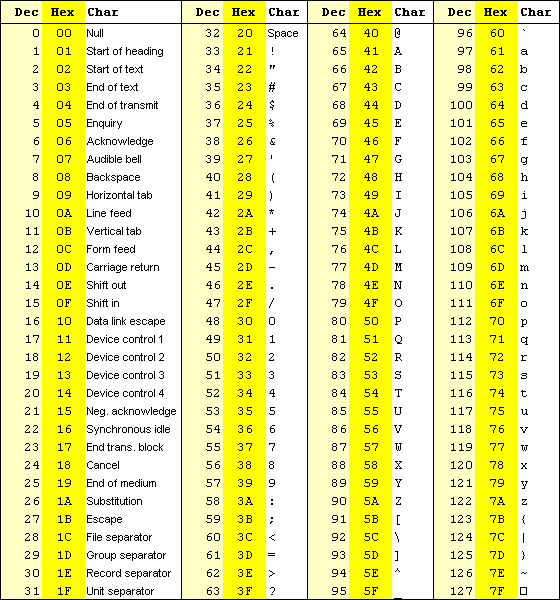
\includegraphics[scale=0.6]{../pictures/ascii}
\caption{The ASCII table. Each number from 0 to 127 refers to a character. The numbers 0 to 31 cannot be printed.}
\label{fig:ascii}
\end{center}
\end{figure}

\begin{figure}
\begin{center}
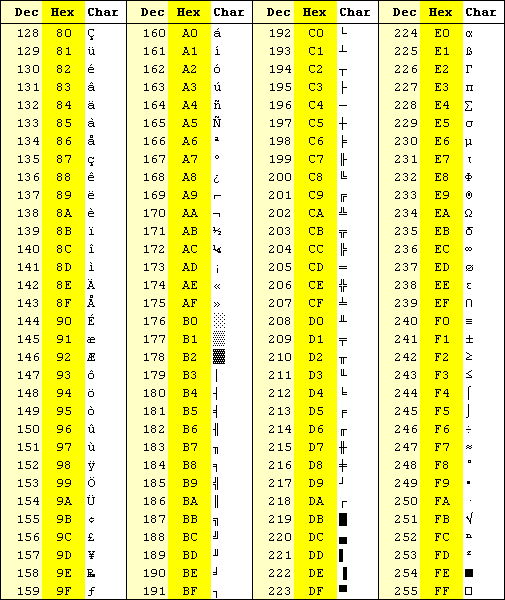
\includegraphics[scale=0.6]{../pictures/ascii2}
\caption{The extended ASCII table. Each number from 128 to 255 refers to a character, mostly special characters not included in the basic table.}
\label{fig:ascii2}
\end{center}
\end{figure}

The application has support for reading common image file formats such as bmp, png and jpg (for a full list, see the supported file formats of the SDL\_image libaray). 8- 16- and 32-bit output is supported, and can be changed by passing a command line argument to the program (by default, the output is adjusted for 16 bit color mode). Both vertical and horizontal grid spacing are set to 32 pixels by default, but this can be changed through command line arguments.

The resulting output header file, which is named after the input, can be included in a program using the bare metal and font driver. The easiest way to use the bitmap font is to use the generated initialize function defined in the header file.

\subsubsection{Mesh maker utility}
\label{sec:meshmaker}
The mesh maker utility loads 3D objects and generates a header file that can be used by the advanced 3D API. Currently the utility only supports Wavefront .obj files which only contains 3rd order polygons. Any higher order polygons will be discarded, so all polygons in the model must be converted to triangles prior to running the utility.

The application supports loading texture coordinates for each vertex, allowing for textured meshes.

The resulting output header file, which is named after the input, can be included in a program using the bare metal 3D API. The easiest way to use the mesh is to use the generated initialize function defined in the header file.

\subsubsection{Vector font maker utility}
\label{sec:fontmaker}
The Font maker is a application that can convert a .ttf file to a format that the graphics card can handle. The Font maker outputs a .h file that can be included in a project to enable the graphics accelerators vector font capabilities. The converter finds all explicit vector points in a ttf file and then calculates the implicit points. At the same time it checks where the glyphs contours ends, the points is then sent to a Delaunay triangulation function based on the work of V. Domiter and B. Zalik and implemented by M. Green and T. \AA hl\'{e}n \footnote{http://code.google.com/p/poly2tri/}. The generated .h file consists of two fields for each glyph, one field for B\'{e}zier writes and one for triangle writes. The generated header file will contain two lists for each glyph, one to store B\'{e}zier writes and one to store triangle writes. The rendered result can be seen in figure \ref{fig:orsocgfxfont}.

\begin{figure}
\begin{center}
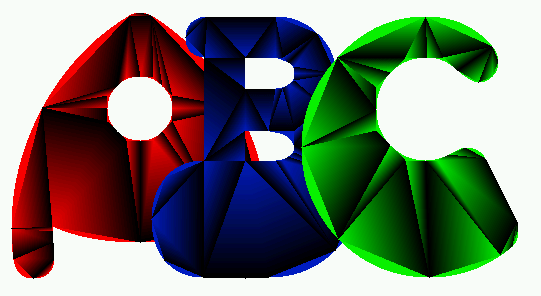
\includegraphics[scale=0.6]{../pictures/orsocgfxfont}
\caption{A font rendered by the software implementation of the ORGFX. B\'{e}zier curves are single colored while the triangles are interpolated between current color and black}
\label{fig:orsocgfxfont}
\end{center}
\end{figure}


\subsubsection{Regger}
The regger is a application that keeps track of what register addresses is set in the RTL code and in the drivers.

\section{Programming examples}
\label{sec:examples}
The following piece of code shows how to use the extended interface for a bare metal implementation on the ORPSoCv2 platform. Bahamut\_cc.png.h is a 186 by 248 pixel image with a pinkish background (rgb code ff00ff, or f81f in 16 bit). The header file is generated by the sprite maker utility at 16 bit color depth.

\begin{lstlisting}
#include "orgfx_plus.h"

#include "Bahamut_cc.png.h"

int main(void)
{
    int i;

    // Initialize screen to 640x480-16@60
    // No double buffering
    int screen = orgfxplus_init(640, 480, 16, 0);

    // Initialize dragon sprite
    int bahamut_sprite =
        orgfxplus_init_surface(186, 248, Bahamut_cc);

    // Activate colorkeying
    orgfxplus_colorkey(0xf81f, 1);

    // Clear screen, white color
    orgfxplus_fill(0,0,640,480,0xffff);
    // Draw a few lines with different colors
    orgfxplus_line(200,100,10,10,0xf000);
    orgfxplus_line(200,100,351,31,0x0ff0);
    orgfxplus_line(200,100,121,231,0x00f0);
    orgfxplus_line(200,100,321,231,0xf00f);
    
    // Draw the dragon at different alpha settings
    orgfxplus_alpha(64,1);
    orgfxplus_draw_surface(100, 100, bahamut_sprite);
    orgfxplus_alpha(128,1);
    orgfxplus_draw_surface(120, 102, bahamut_sprite);
    orgfxplus_alpha(255,1);
    orgfxplus_draw_surface(140, 104, bahamut_sprite);

    while(1);
}
\end{lstlisting}

More example programs are supplied with the implementation in the \textbf{sw/examples} directory.

\end{document}
